\lesson{7}{06.11.2023}{Прямые на плоскости. Плоскости в пространстве}

\section{Угол между прямыми}

\begin{definition}[Угол между прямыми]
    Даны прямые $l_1, l_2$:
    \begin{gather*}
        l_1: a_1x +b_1y + c_1 = 0\\
        l_2: a_2x +b_2y + c_2 = 0\\
        \angle(l_1, l_2) = \angle (\vn_1, \vn_2)\\
        \cos \angle(l_1, l_2) = \frac{a_1a_2+b_1b_2}{\sqrt{a_1^2 + b_1^2} + \sqrt{a_2^2 + b_2^2}}\\
        l_1 \perp l_2 \Leftrightarrow a_1 a_2 + b_1 b_2 = 0\\
        l_1 \parallel l_2 \Leftrightarrow \frac{a_1}{a_2} = \frac{b_1}{b_2}
    \end{gather*}  
\end{definition}



\begin{definition}(другое определение)
    \begin{gather*}
        l_1: \frac{x-x_0}{v_1}=\frac{y-y_0}{v_2} \qquad l_2: \frac{x-x_1}{w_1} = \frac{y-y_1}{w_2}\\
        \vv = (v_1, v_2) \qquad \vw = (w_1, w_2)\\
        \cos \angle(l_1, l_2) = \frac{v_1 w_1 + v_2 w_2}{\sqrt{v_1^2 + v_2^2}\sqrt{w_1^2 + w_2^2}}\\
        l_1 \perp l_2 \Leftrightarrow v_1 w_1 + v_2 w_2 = 0\\
        l_1 \parallel l_2 \Leftrightarrow \frac{v_1}{w_1} = \frac{v_2}{w_2}
    \end{gather*}
\end{definition}

\section{Уравнение нормали}

\begin{definition}
    $(a,b) = \vn$ называется вектором нормали к прямой
    \begin{gather*}
        ax+by+c=0 \qquad |:\sqrt{a^2 + b^2}\\
        a'x+b'y +c' = 0 \text{ -- Нормальное уравнение прямой}\\
        a'^2 + b'^2 = 1 \qquad a' = \frac{a}{\sqrt{a^2 + b^2}} \qquad b' = \frac{b}{\sqrt{a^2 + b^2}}\\
        (a', b')\text{ -- единичный вектор }
    \end{gather*}
    
    
    $|c'| = |\frac{c}{\sqrt{a^2+b^2}}|$ -- расстояние от начала координат до прямой. (?)\\
    $(a', b')$ называют направляющими косинусами, т.к.
    \begin{center}
        \begin{tikzpicture}[scale=3]
            \draw[very thick, -Latex] (-0.3, 0) -- (0.7, 0) node(xline) [right] {$x$};
            \draw[very thick, -Latex] (0, -0.3) -- (0, 0.7) node(yline) [above] {$y$};
            \draw[-Latex] (0,0)--(0.5, 0.3) node[right] {$\vn = (a', b')$};
            \draw (0.1, 0.2) node {$\beta$};
            \draw (0.2, 0.05) node {$\alpha$};
        \end{tikzpicture}
    \end{center}
    \begin{gather*}
        |\vn| = 1 \qquad a'^2 + b'^2 = 1\\
        a' = \cos \alpha\\
        b' = \sin \alpha = \cos \beta
    \end{gather*}
\end{definition}

\begin{theorem}
        Hасстояние от точки $(x_1, y_1)$ до прямой $ax+by+c=0$ -- это
              \[d = \frac{|ax_1 + by_1 +c|}{\sqrt{a^2 + b^2}}\]
\end{theorem}
\begin{proof}
    $M + \lambda \vn \in l$ -- прямая $\vn$ -- нормаль (a, b)

    \begin{tikzpicture}[scale=3, xscale=-1]
        \draw[blue] (-0.3, 1)node[above] {$l$} -- (1.3, -0.3);
        \draw[Latex-] ($(-0.3, 1)!(0,0)!(1.3, -0.3)$) node[above, left] {$\lambda \vn$} -- (0,0);
        \draw[shorten <=0.5cm, red, Latex-] ($(-0.3, 1)!(0,0)!(1.3, -0.3)$) --
        node[right] {$\vn$} (0,0);
        node[dot] (M) at (0.5,0.5) {};
        node[right] at (M) {$M$};
    \end{tikzpicture}

    $$\dist (M, l) = |\lambda| \cdot |\vn| \text{ из рисунка}$$
    $$M + \lambda \vn = (x_0 + \lambda a, y_0 + \lambda b) \in l \implies a(x_0 \lambda a) + b(y_0 + \lambda b) + c = 0$$
    $$ax_0 + by_0 + c + \lambda (a^2 + b^2) = 0 \implies \lambda = -\frac{(ax_0 + by_o + c)}{a^2+b^2}$$
    $$\text{тогда } |\lambda| \cdot |\vn| = |-\frac{(ax_0 + by_o + c)}{a^2+b^2}| \cdot |\sqrt{a^2+b^2}| = |\frac{(ax_0 + by_o + c)}{\sqrt{a^2+b^2}}|$$
\end{proof}

\section{Уравнение прямой, проходящей через точку пересечения двух других}

\begin{definition}
    Есть 2 прямые: $l_1: a_1x + b_1y + c_1 = 0$ и $l_2: a_2x + b_2y + c_2 = 0$ и точка $M$ -- точка пересечения. Тогда $\exists \lambda_1, \lambda_2:$

    \[l_3: \lambda_1(a_1x + b_1y + c_1) + \lambda_2(a_2x + b_2y + c_2) = 0 \text{ прямая, проходящая через М}\]

    Эта прямая проходит через М, т.к. при подстановке координат М в уравнение, первое и второе слагаемые обращаются в 0. 
\end{definition}

\chapter{Плоскости в пространстве}

\section{Уравнение плоскости}

$\dim V = 3$
\begin{definition}[Плоскость по 3 точкам]
    Пусть $e_1, e_2, e_3 \in E$, $\vv_1 = \overrightarrow{e_1 e_2}; \vv_2 = \overrightarrow{e_1 e_3}$

    Плоскость -- множество точек $\{e_1 + \alpha\vv_1 + \beta \vv_2: \alpha, \beta \in \R\}$
\end{definition}
\begin{definition}
    Плоскость -- множество решений линейного уравнения:
    \[Ax + By +Cz + D = 0\]
\end{definition}
\begin{theorem}
    Определение 1 равносильно определению 2.
\end{theorem}
\begin{theorem}
    $(A,B,C) = \vn \perp \text{ плоскости}$
\end{theorem}
\begin{proof}
    \begin{gather*}
        e_1 = (x_0, y_0, z_0)\\
        \vn \perp \vv_1 \qquad \vn \perp \vv_2 \qquad \vn = \vv_1 \times \vv_2 \qquad \vn = (A,B,C)\\
        \intertext{$D$ такое число, что}
        Ax_0 + By_0 + Cz_0 + D = 0 \qquad (D = -Ax_0 - By_0 - Cz_0)\\
        - \begin{array}{l}
            Ax + By + Cz + D = 0       \\
            Ax_0 + By_0 + Cz_0 + D = 0 \\
        \end{array}\\
        \begin{array}{l}
            \hline
            A(x - x_0) + B(y - y_0) + C(z - z_0) = 0
        \end{array}\\
        (A;B;C) \cdot (x-x_0, y-y_0, z-z_0) = 0\\
        (x-x_0, y-y_0, z-z_0) = \alpha \vv_1 + \beta \vv_2\\
        (x,y,z) = e_1 + \alpha \vv_1 + \beta \vv_2 \qedhere
    \end{gather*}
\end{proof}

\begin{definition}[Нормальное уравнение плоскости]
    \begin{gather*}
        Ax + By + Cz + D = 0 \qquad |:\sqrt{A^2 + B^2 +C^2} \neq 0\\
        A'x + B'y + C'z +D' = 0\\
        A'^2 + B'^2 + C'^2 = 1
    \end{gather*}
\end{definition}

$A', B', C'$ -- направляющие косинусы




\noindent\begin{minipage}{.45\textwidth}
    \begin{center}
        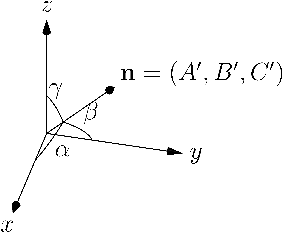
\includegraphics{directional_cosines.pdf}
    \end{center}
\end{minipage}
\begin{minipage}{.45\textwidth}
    \begin{gather*}
        A' = \cos \alpha\\
        B' = \cos \beta\\
        C' = \cos \gamma\\
    \end{gather*}
\end{minipage}

\begin{theorem} (доказательство аналогично прямой на плоскости)
            Пусть $Ax + By + Cz + D = 0$ -- плоскость, а $(x_0, y_0, z_0)$ -- точка,
              тогда расстояние от точки до плоскости:
              \[d = \frac{|Ax_0 + By_0 + Cz_0 + D|}{\sqrt{A^2 + B^2 + C^2}}\]
\end{theorem}

\begin{definition}[Уравнение плоскости в отрезках]
    \[\frac{x}{p} + \frac{y}{q} + \frac{z}{r} = 1\]
    $p,q,r$ -- отрезки высекаемые плоскостью на $OX, OY, OZ$
\end{definition}


\section{Угол между плоскостями}

\begin{definition}[Угол между плоскостями]
    \begin{gather*}
        A_1x + B_1 y + C_1 z + D_1 = 0 = \alpha_1\\
        A_2x + B_2 y + C_2 z + D_2 = 0 = \alpha_2\\
        \cos\angle(\alpha_1, \alpha_2) =
        \frac{A_1 A_2 + B_1 B_2 + C_1 C_2}{\sqrt{A_1^2 + B_1^2 + C_1^2}\sqrt{A_2^2 + B_2^2 + C_2^2}}\\
        \alpha_1 \perp \alpha_2: A_1 A_2 + B_1 B_2 + C_1 C_2 = 0\\
        \alpha_1 \parallel \alpha_2: \frac{A_1}{A_2} = \frac{B_1}{B_2} = \frac{C_1}{C_2}
    \end{gather*}
\end{definition}

\section{Плоскость через прямую пересечения двух плоскостей}

\begin{definition}
    \begin{gather*}
        \alpha_1: A_1x + B_1 y + C_1 z + D_1 = 0\\
        \alpha_2: A_2x + B_2 y + C_2 z + D_2 = 0\\
        \alpha_3: \lambda_1(A_1x + B_1 y + C_1 z + D_1) + \lambda_2(A_2x + B_2 y + C_2 z + D_2) = 0
    \end{gather*}
\end{definition}

\section{Плоскость через точку пересечения трех плоскостей}

\begin{definition}
    \begin{gather*}
        \alpha_1: A_1x + B_1 y + C_1 z + D_1 = 0\\
        \alpha_2: A_2x + B_2 y + C_2 z + D_2 = 0\\
        \alpha_3: A_3x + B_3 y + C_3 z + D_3 = 0\\
        \alpha_4: \lambda_1(A_1x + \ldots + D_1) + \lambda_2(A_2x + \ldots + D_2) + \lambda_3(A_3x + \ldots + D_3) = 0
    \end{gather*}
\end{definition}

\chapter{Прямая в пространстве}

\section{Уравнение прямой}

\begin{definition}
    Прямая -- пересечение двух не параллельных плоскостей.
\end{definition}


\begin{definition}[Каноническое уравнение прямой в пространстве]
    Если есть $(x_0, y_0, z_0)$ и $(x_1, y_1, z_1)$, то прямая через эти точки задается уравнением:
    \[\frac{x-x_0}{x_1-x_0} = \frac{y-y_0}{y_1-y_0} = \frac{z-z_0}{z_1-z_0}\]
\end{definition}

\begin{definition}[Каноническое уравнение прямой в пространстве]
    Если есть 2 уравнения плоскости, то прямая задается как
    \begin{gather*}
        \begin{cases}
            A_1 x + B_1 y + C_1 z + D_1 = 0 \\
            A_2 x + B_2 y + C_2 z + D_2 = 0
        \end{cases}\\
        \vn_1 = (A_1, B_1, C_1) \qquad \vn_2 = (A_2, B_2, C_2)\\
        \vv \perp \vn_1 \qquad \vv \perp \vn_2 \qquad \vv = \vn_1 \times \vn_2\\
        \vv = (v_1, v_2, v_3)\\
        \frac{x-x_0}{v_1} = \frac{y-y_0}{v_2} = \frac{z-z_0}{v_3}
    \end{gather*}
\end{definition}

\begin{definition}
    $\vv = (v_1, v_2, v_3)$ -- направляющий вектор
\end{definition}

\begin{definition}[Параметрическое уравнение прямой в пространстве]
    \[
        \frac{x-x_0}{v_1} = \frac{y-y_0}{v_2} = \frac{z-z_0}{v_3} = t \Leftrightarrow
        \begin{cases}
            x = x_0 + v_1 t \\
            y = y_0 + v_2 t \\
            z = z_0 + v_3 t
        \end{cases}
    \]
\end{definition}

\begin{theorem}
    Любая прямая -- прямая пересечения двух непараллельных плоскостей, и наоборот.
\end{theorem}

\begin{proof}
    $\newline$
    \begin{itemize}
        \item[$\Rightarrow:$] каноническое уравнение: 
        
        $\begin{cases}
            \frac{x-x_0}{v_1} = \frac{y-y_0}{v_2} \text{ -- плоскость} \\
            \frac{y-y_0}{v_2} = \frac{z-z_0}{v_3} \text{ -- плоскость}
        \end{cases}$
        
        \item[$\Leftarrow:$] пусть есть 2 плоскости: 
        
        $\begin{cases}
            A_1 x + B_1 y + C_1 z + D_1 = 0 \\
            A_2 x + B_2 y + C_2 z + D_2 = 0
        \end{cases} \implies \begin{cases}
            x = x_0 + v_1 z \\
            y = y_0 + v_2 z \\
        \end{cases} \implies $
        $$\implies \frac{x-x_0}{v_1} = \frac{y-y_0}{v_2} = \frac{z-z_0}{v_3}$$
    \end{itemize}
\end{proof}